\PassOptionsToPackage{patch=none}{microtype}
\documentclass[sigconf,nonacm]{acmart}

\settopmatter{printacmref=false, printccs=false, printfolios=true}
\renewcommand\footnotetextcopyrightpermission[1]{} 
\pagestyle{plain}

\usepackage{geometry}
\geometry{top=0.7in, bottom=1in, left=0.75in, right=0.75in}
\usepackage[T1]{fontenc}
\usepackage{newtxtext,newtxmath}
\usepackage{booktabs}
\usepackage{enumitem}

\makeatletter
\renewcommand{\section}{\@startsection{section}{1}{\z@}%
  {-3.5ex \@plus -1ex \@minus -.2ex}%
  {2.3ex \@plus.2ex}%
  {\reset@font\Large\bfseries}}
\renewcommand{\subsection}{\@startsection{subsection}{2}{\z@}%
  {-3.25ex\@plus -1ex \@minus -.2ex}%
  {1.5ex \@plus .2ex}%
  {\reset@font\large\bfseries}}
\makeatother

\graphicspath{{../proposal/}, {../algorithm/}}
\renewcommand{\UrlFont}{\ttfamily}

\begin{document}

\setlist[enumerate,1]{leftmargin=*}
\setlist[itemize,1]{leftmargin=*}

\title{Solving enclose.horse to Optimality via Multi-Commodity Flow Integer Linear Programming Reduction}

\author{Kyle Trinh, Stefan Gadient, Aston Du, Elena Tomson, Özgür Özerdem}
\affiliation{%
  \institution{University of California, San Diego}
  \city{La Jolla}
  \state{California}
  \country{USA}
}
\email{{kytrinh, sgadient, asdu, etomson, oozerdem}@ucsd.edu}

\newcommand{\horse}{\href{https://enclose.horse}{\texttt{enclose.horse}}}
\newcommand{\level}[1]{\href{https://enclose.horse/play/#1}{{\color{blue}\texttt{#1}}}}

\begin{abstract}
  Our project implements an Integer Linear Programming (ILP) solver for \horse. We detail the formulation, optimizations, and results of benchmarking against 72 daily puzzles and 12,689 custom puzzles. The solver find the optimal solution for 100\% of the daily puzzles, and matches or exceeds human performance in over 99.2\% of the custom puzzles, sometimes identifying optimal configurations that improve upon existing leaderboard records.
\end{abstract}

\maketitle

\section{Introduction}

\horse\ is a grid-based puzzle game where the player must enclose a horse within a pen using a limited budget of $k$ walls. The grid consists of various tile types, each contributing to the total score if contained within the enclosed region. Standard grass tiles, portals, and the horse's starting position each have a base value of 1 point. Special point modifiers include cherries (+3 bonus points, 4 total), golden apples (+10 bonus points, 11 total), and bee swarms ($-5$ points penalty, $-4$ total).

The primary constraint is that there must be no path from the horse to the grid boundary (escapability). Water tiles act as natural, impassable barriers where walls cannot be placed. Portals come in pairs and provide non-local connectivity, allowing the horse to teleport between them. The objective is to select a subset of empty grass tiles for wall placement that maximizes the sum of values for all reachable tiles while adhering to the wall budget $k$. We reduce this optimization problem to an ILP problem using binary variables for wall placement ($\mathbf{W}$), escapability ($\mathbf{E}$), and reachability ($\mathbf{R}$), with commodity flow constraints to ensure the connectivity of the enclosed pen. Our approach is inspired by the ILP reduction proposed by Dynomight \cite{dynomight}, which we extend to support advanced mechanics and size-constrained connectivity \cite{CHEN2016434}.

\section{Algorithm Description}

Our approach reduces \horse\ to an ILP problem using three binary matrices for an $L \times W$ grid: wall placement ($\mathbf{W}$), escapability ($\mathbf{E}$), and horse-reachability ($\mathbf{R}$).

\subsection{Connectivity and the Adversarial Case}
A baseline algorithm that simply minimizes escapable tiles, as described in \cite{dynomight}, fails when the solver creates enclosed regions disconnected from the horse.
 Since the game score only counts tiles reachable by the horse, these ``adversarial rooms'' yield suboptimal results. To ensure a single connected component, we implement a commodity flow constraint. We define the horse as a source of flow $M = \sum \mathbf{R}[i,j]$. Each tile $(i,j)$ is reachable ($\mathbf{R}[i,j]=1$) if and only if it consumes exactly one unit of flow from the horse. This formulation prevents isolated islands of enclosed space from being erroneously counted toward the objective.

\subsection{Portals and Point Modifiers}
Portals provide non-local connectivity. For a portal pair $(p, q)$ where $p$ and $q$ are coordinate locations of portals, we enforce $\mathbf{R}[p] = \mathbf{R}[q]$ and $\mathbf{E}[p] = \mathbf{E}[q]$, allowing reachability and escapability to propagate across the grid. Point modifiers are incorporated via a value function $\mathbf{F}[i,j]$, where $\mathbf{F}[i,j] \in \{1, 4, 11, -4\}$ based on the tile type. The objective function is defined as $\max \sum \mathbf{R}[i,j] \cdot \mathbf{F}[i,j]$, ensuring the solver prioritizes enclosing high-value items while avoiding bee swarms.

\subsection{Linearization and Optimizations}
Our first draft of the algorithm design inadvertently included constraints which incorporated the product of multiple variables, which is nonlinear and thus invalid for linear programming. However, we were able to linearize these constraints in our implementation to accommodate standard solvers. For instance, interior escapability is now defined as $\mathbf{E}[i,j] \geq \mathbf{E}[i',j']-\mathbf{W}[i,j]$ instead of $\mathbf{E}[i,j] \geq (1 - \mathbf{W}[i,j]) \cdot \mathbf{E}[i',j']$ for $(i',j')$ neighbors of $(i,j)$. We also introduced some optimizations to improve performance from our original algorithm:
\begin{enumerate}
    \item \textbf{Variable Consolidation.} In our original approach, we related the matrices $\mathbf{W},\mathbf{E},\mathbf{R}$ to each other in a number of different constraints, all essentially saying that a tile could either be a wall, escapable, or reachable (or none of these) but not more than one. In our implementation, we consolidate all these constraints into the single constraint of $\mathbf{W}[i,j]+\mathbf{E}[i,j]+\mathbf{R}[i,j] \leq 1$, ensuring each tile occupies exactly one state and improving LP relaxation pruning.
    \item \textbf{Sparsity Filtering.} Water tiles and the horse's tile are already required to have predetermined values of $\mathbf{W},\mathbf{E},\mathbf{R}$. Namely, water tiles cannot have a wall, be escapable, or be reachable; and the horse cannot have a wall or be escapable, but must be reachable. Therefore, in order to reduce the ILP problem's dimensionality, decision variables for water tiles and the horse position are pre-assigned instead of being computed by the solver.
\end{enumerate}

\section{Theorems and Complexity}

We claim that the \horse\ problem is NP-complete. To show this, we must show that the problem is in NP and that it is NP-hard.

\subsection{Problem is in NP}

Let $S \in \mathcal{E}$ be a solution to an instance of the \horse\ problem. We can verify that $S$ is a valid solution in polynomial time by counting the number of fences and checking that it is at most $k$, and then cutting the $k$ vertices from the graph $G$, and finally run a modified BFS to check that the horse is enclosed and to calculate the score of the pen. All of these steps can be done in polynomial time, so the problem is in NP.

\subsection{Problem is NP-hard}

We claim the minimum s-t edge cut problem of size at most $T$ can be reduced to the \horse\ problem.
The minimum s-t edge cut problem is defined as follows: given a graph $G$ and two vertices $s$ and $t$, determine the minimum number of edges that must be removed from $G$ to disconnect $s$ from $t$ such that the number of vertices reachable from $s$ is at least $T$. This problem is known to be NP-complete \cite{CHEN2016434}.

We now show the reduction from the minimum s-t edge cut problem of size at least $T$ to the \horse\ problem. Given an instance of the minimum s-t edge cut problem (G, $s$, $t$, $T$), we can construct an instance of the \horse\ problem as follows: we create a grid graph $G$ where each vertex corresponds to a cell in the grid. We place the horse at vertex $s$, $O$ at vertex $t$, and for each vertex $v$ in $G$, we add a vertex which is not fence placable with weight 1 to the grid graph. For each edge $(u, v)$ in $G$, we add an auxilary vertex $v_e$ which is fence-placable with weight 0, and we add edges $(u, v_e)$ and $(v_e, v)$ to the grid graph. Then, we perform binary search on the value of $k$ to find the minimum $k$ such that there exists a solution to the \horse\ problem with score at least $T$. The graph construction takes polynomial time, and the binary search takes $O(\log |E|)$, so the reduction is polynomial time.

\section{Implementation and Experiments}

% The experimental framework is implemented as the \texttt{enclose\_engine} Python package, a modular suite designed for both interactive gameplay and large-scale benchmarking. The core logic in \texttt{engine.py} handles tile-level mechanics and graph-based reachability, while the solving logic is decoupled into specialized ILP classes.

The experimental framework is implemented in Python 3.14.3. We designed a simple game engine to help us visualize and debug the solver, while the solver itself creates an ILP model using the constraints defined in the algorithm description and passes it to \texttt{PuLP}.

\subsection{Solver Iterations}
The solver went through four distinct phases as we attempted to implement global connectivity and optimize efficiency:
\begin{itemize}
    \item \textbf{Baseline (\texttt{solver.py}):} A local escapability propagation model that lacked global connectivity constraints, often yielding invalid ``island'' pens.
    \item \textbf{Version 2 (\texttt{Alt2}):} The first to integrate commodity flow logic. However, it still failed to properly propogate reachability, so the solver would set $R[i,j]=0$ for bee tiles without ensuring that those tiles are not reachable. It also suffered from high variable redundancy on large grids ($O(N^2)$ flow variables).
    \item \textbf{Version 3 (\texttt{Alt3}):} The first fully correct solver, fixed reachbility logic and focused on portal normalization. By deduplicating portal graph edges, we eliminated variable name collisions in the \texttt{PuLP} model and prevented flow cycles that previously caused solver instability.
    \item \textbf{Version 4 (\texttt{Alt4}):} The final production solver, focused on reducing total number of variables to optimize runtime. It employs sparsity filtering to exclude non-placeable tiles (water, horse) from the variable pool and strengthens the LP relaxation by consolidating state transitions into a single mutual exclusion constraint, as described above.
\end{itemize}

In our provided code, the \texttt{Alt4} solver is implemented as merely the solver.py file, and the other versions were removed.

\subsection{Experimental Pipeline and Setup}
We built a web scraper to acquire 72 daily and 12689 custom puzzles from the \horse\ API, targeting all daily challenges and all community levels with $\geq 5$ plays. To create our scraper, we used browser developer tools to inspect the API calls for games being loaded in the website's Browse page, reverse engineered the API call parameters, and wrote a script to scrape all games on the site, sorted by highest play count over all time. We then took all games with at least 5 plays. We ran the scraper on 11 March 2026, so leaderboard data and reported optimal scores for benchmarking come from this date. Benchmarking was performed on dual AMD EPYC 7713 64-Core Processors (256 logical threads) with 1~TB of RAM.

To maximize hardware utilization, we implemented a parallel execution strategy using a \texttt{ProcessPoolExecutor} running 25 concurrent \texttt{CBC} instances. Each instance was allocated 10 threads and a 120s timeout. In case the \texttt{CBC} instance did not timeout for whatever reason, we implemented a hard limit of 140s, immediately killing the thread if passed. This approach allowed us to process the entire 12,689 puzzle set in approximately 25 minutes, representing a cumulative compute effort of over 100 CPU-hours. For the most complex cases that exceeded this threshold, we performed extended reruns using a deep-search configuration with 32 threads per instance.

\section{Performance}

The average difficulty of the daily puzzles is significantly lower than that of the custom puzzles, allowing our model to solve 100\% of the daily puzzles within a 10 second threshold. The total benchmark took approximately 120 seconds, with a mean daily puzzle solve of time <2 seconds. So we instead focus on performance metrics for the custom puzzles, which are more representative of the solver's capabilities and limitations. Performance metrics for the primary custom puzzle benchmark with a limit of 120s/puzzle are summarized in Table~\ref{tab:bench}.

\begin{table}[h]
  \centering
  \caption{Benchmarking Summary (n=12,689)}
  \label{tab:bench}
  \begin{tabular}{lrr}
    \toprule
    Result Category & Count & Percentage \\
    \midrule
    Matched Optimal Score & 11,911 & 93.87\% \\
    Surpassed Optimal Score & 676 & 5.33\% \\
    Sub-Optimal Score (Non-Timeout) & 7 & 0.06\% \\
    Timed Out ($>$120s) & 95 & 0.74\% \\
    \bottomrule
  \end{tabular}
\end{table}

The solver improved upon the reported ``optimal'' scores in 5.33\% of puzzles. (Note that for community-submitted levels, which comprise the vast majority of the benchmarking puzzles, the ``optimal'' score is merely the highest score that a user had achieved at the time of scraping.) These improvements often occured on maps with complex portal networks, which anecdotally is extremely difficult for human players to optimize on. The initial benchmarking also identified 7 maps where our solver apparently terminated without finding the optimal score, which appear to (but do not actually) present critical failures of our algorithm; we discuss these later.


% \subsection{Human Heuristics vs. Global Optimality}
% The solver improved upon the reported "optimal" scores in 5.33\% of puzzles. These improvements often occur on maps with complex portal networks where human players fail to identify non-local packing opportunities. This confirms that human heuristics are often limited to local boundary-following, whereas the ILP explores the full modifier trade-off space.

To maintain the integrity of our benchmarking, we refrained from submitting any solutions to the \horse\ leaderboards during development, ensuring that our reported optimal scores reflect the state of the art at the time of scraping.

\subsection{Long-Tail Complexity and Convergence}
The distribution of solve times (Table~\ref{tab:dist}) shows that while the median case is trivial, the worst-case complexity grows significantly. We illustrate this table in Figure~\ref{fig:cdf}. 

\begin{table}[h]
  \centering
  \caption{Solve Time Distribution (Optimal \& No Timeout, n=12,583)}
  \label{tab:dist}
  \begin{tabular}{lr}
    \toprule
    Percentile & Solve Time (s) \\
    \midrule
    50\% (Median) & 0.354 \\
    90\% & 4.291 \\
    99\% & 30.432 \\
    Max (Rerun) & 4,617.175 \\
    \bottomrule
  \end{tabular}
\end{table}

\begin{itemize}
    \item \textbf{Phase Transition:} Scatter plots of solving time versus number of empty fields show a distinct computational phase transition around 600 fields. While 99.2\% of puzzles solve within the 120s threshold, levels exceeding this threshold require a prohibitively long time to solve.
    \item \textbf{Extreme Cases:} Extended reruns of timed-out levels using 32 threads (Table~\ref{tab:hardness}) revealed that puzzles such as \level{lzhqD7} and \level{BYPcZO} can require over an hour to prove optimality. We observed that timeouts were most frequent on large grids ($15\times15$ to $30\times30$) that were almost or completely empty but provided a large wall budget. In these sparse configurations, the combinatorial explosion of potential wall placements maximizes the search tree depth.
\end{itemize}

We also attempted to find correlations between solve time and other level features such as number of bees, flowers, and portals, but found no significant linear relationships. This suggests that the solver's performance is more sensitive to the combinatorial structure of the solution space rather than specific modifier counts. However, one thing to note is that grid size and wall budget were somewhat correlated with solve time as shown in Figure~\ref{fig:scatter}, which is consistent with our observation that large, nearly-empty grids are the most difficult to solve. 

\begin{table}[h]
  \centering
  \caption{Computational Hardness Benchmark (Extended Reruns)}
  \label{tab:hardness}
  \begin{tabular}{lrrr}
    \toprule
    Game ID & Grid Size & Wall Budget & Solve Time (s) \\
    \midrule
    \level{nxko1o} & $30\times30$ & 20 & 1,427.76 \\
    \level{oWidWC} & $30\times30$ & 20 & 2,072.62 \\
    \level{BYPcZO} & $30\times30$ & 50 & 4,356.06 \\
    \level{lzhqD7} & $30\times30$ & 50 & 4,617.18 \\
    \bottomrule
  \end{tabular}
\end{table}


\begin{figure}[h]
  \centering
  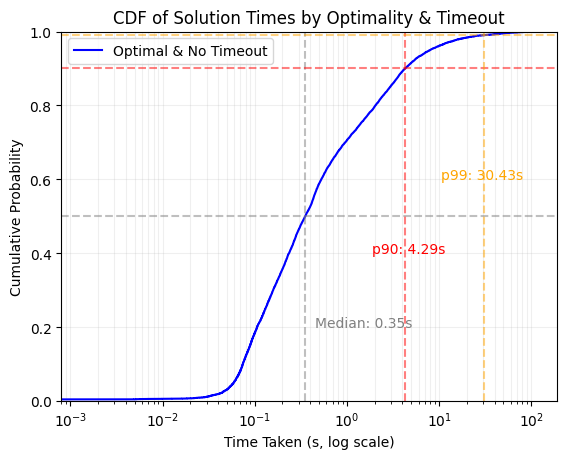
\includegraphics[width=\linewidth]{cdf.png}
  \caption{CDF of Solve Times for Optimal Solutions (n=11,911)}
  \label{fig:cdf}
\end{figure}

\begin{figure}[h]
  \centering
  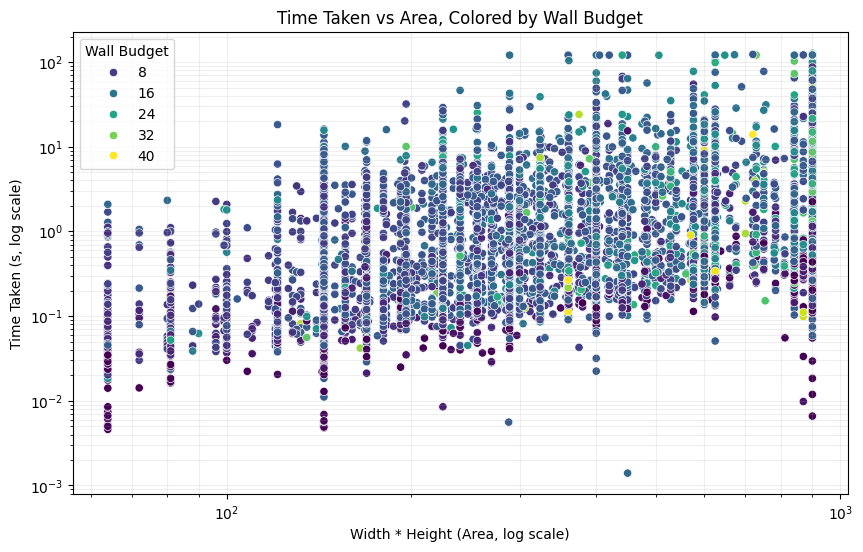
\includegraphics[width=\linewidth]{area.png}
  \caption{Scatter Plot of Solve Time vs. Area, Wall Budgets $\leq 50$ (n=12,583)}
  \label{fig:scatter}
\end{figure}

\subsection{Failure Analysis}
Games where the solver terminated but returned suboptimal results (7 games) were manually reviewed. In every case, the reported score was found to be impossible to achieve, which we attribute to discrepancies in the game's leaderboard API. In particular, each offending level had a reported optimal score of 0, but the actual optimal score was in the negatives (due to bee swarms being forced to be included in any valid solution). These levels were: \level{0LV\_O-}; \level{A5YZ6C}; \level{DeAMwX}; \level{Ft-to2}; \level{LCHDaM}; \level{e\_bX\_I}; and \level{vsBDjp}. Of the 95 remaining puzzles in the original benchmarking that failed to match the optimal score, all were due to the 120s timeout; these puzzles were successfully solved in the extended reruns.

% \subsection{Bee Swarm Robustness}
% Bee swarms create a penalty trade-off that test the solver's modifier handling. As shown in Table~\ref{tab:modifiers}, the flow-based model is highly robust, achieving perfect accuracy on levels without modifiers and near-perfect accuracy on levels with penalties.

% \begin{table}[h]
%   \centering
%   \caption{Solver Robustness by Modifier Presence}
%   \label{tab:modifiers}
%   \begin{tabular}{lrr}
%     \toprule
%     Modifier Category & Count & Accuracy (No Timeout) \\
%     \midrule
%     Levels with Bees & 4,062 & 99.83\% \\
%     Levels without Bees & 8,627 & 100.00\% \\
%     \bottomrule
%   \end{tabular}
% \end{table}

\section{Conclusion}

Our project successfully reduced the $\horse$\ puzzle game to an Integer Linear Programming problem using a multi-commodity flow formulation. We developed a solver that guarantees optimal pen configurations. 

Our empirical evaluation against 12,689 puzzles demonstrates that the \texttt{Alt4} optimizations—specifically sparsity filtering and strengthened mutual exclusion—allow for sub-second median convergence on standard grids. Future work might explore optimizations for cases like large, nearly-empty grids, which accounted for most of the timeout levels.
% Future work will explore the integration of this solver into real-time puzzle design tools to evaluate level difficulty and modifier balance automatically.

\begin{acks}
The authors thank the CSE 202 staff for guidance on ILP reductions and the creator of \horse\ for the platform. We also thank Patryk Tomalak for providing compute resources during the benchmarking phase. 
\end{acks}

\nocite{*}
\bibliographystyle{plain}
\bibliography{refs}

\end{document}
